\documentclass[10pt]{article}

\usepackage[margin=1in]{geometry}
\usepackage{amsmath,amssymb}
\usepackage{booktabs}
\usepackage{graphicx}
\usepackage{hyperref}
\usepackage{xcolor}

\graphicspath{{figures/}}
\hypersetup{colorlinks=true, linkcolor=blue, citecolor=blue, urlcolor=blue}

\title{Best-of-N or Tree Search?\\A Controlled Study of Learned-Dynamics Optimism Under Test-Time Planning}
\author{Jason Wang}
\date{\today}

\begin{document}
\maketitle

\begin{abstract}
Tree search over a learned dynamics model is usually framed as planning. This note studies a complementary view: search is also a test-time optimizer over the learned model, and can therefore amplify learned-model errors. We build a controlled continuous-control point-mass task with a localized optimistic ``bias pocket'' in the learned dynamics and reward surrogate. Static best-of-N evaluates independent rollouts, while MCTS adaptively expands and backs up branches that look valuable under the model. In a repeated-seed full run, UCT MCTS exhibits a larger selected-return optimism gap than best-of-N at the largest tested forward-model budget, and uncertainty-calibrated search reduces the gap below both. The contribution is not a robotics benchmark result; it is a compact mechanism testbed for studying when adaptive planning improves behavior and when it concentrates compute on model optimism.
\end{abstract}

\section{Motivation}

Learned model-based agents such as PlaNet \cite{hafner2019planet}, Dreamer \cite{hafner2020dreamer}, and PETS \cite{chua2018pets} demonstrate that learned dynamics can support efficient control. MCTS variants are also being extended to imperfect or continuous transition models \cite{kohankhaki2024transition,riviere2024sets}. At the same time, recent test-time compute work has sharpened the distinction between static best-of-N sampling and adaptive search against a learned scorer \cite{snell2024testtime}.

This repository connects those views. If a learned dynamics model is also the test-time evaluator, then MCTS is an optimizer over a fallible model. More compute can improve planning, but it can also increase exposure to localized optimism. The goal is to make that effect measurable in a small setting before moving to larger robotics tasks.

\section{Controlled Mechanism}

The environment is a deterministic 2D point robot. The true reward encourages progress to a goal, penalizes action cost, and mildly penalizes an off-route pocket. The learned surrogate is accurate almost everywhere but, near that pocket, it predicts extra reward and a transition drift toward the goal. It also reports elevated uncertainty in that region.

For a selected action sequence \(a_{0:H-1}\), we measure
\[
\Delta_{\mathrm{opt}} =
  \hat G(a_{0:H-1}) - G(a_{0:H-1}),
\]
the learned-model return minus the true rollout return for the same sequence. We also record cumulative reward bias, transition error, uncertainty exposure, root visit concentration, and depth-wise bias.

\section{Planners}

The planner suite uses the same discrete action set and forward-model budget accounting:

\begin{itemize}
    \item \textbf{Random open loop}: one random sequence.
    \item \textbf{Best-of-N}: independent model rollouts, selecting the maximum learned return.
    \item \textbf{UCT MCTS}: adaptive expansion with UCB selection and discounted backups.
    \item \textbf{Value MCTS}: MCTS with a learned leaf value estimate.
    \item \textbf{Uncertainty MCTS}: subtracts an uncertainty penalty during model scoring.
    \item \textbf{Conservative MCTS}: subtracts uncertainty during backup.
\end{itemize}

The intended repair is a lower-confidence search target. If uncertainty \(u(s,a)\) upper-bounds local optimism, then replacing \(\hat r\) with \(\hat r - \lambda u\) in search or backup can suppress the branch before it dominates the root statistics.

\section{Results}

The full run uses 20 seeds and five budgets from 64 to 1024. The headline artifact is saved in \path{results/full/manifest.json}. At budget 1024, the selected-return optimism gap is larger for UCT MCTS than for static best-of-N, while the best calibrated repair reduces the gap:

\begin{table}[h]
\centering
\begin{tabular}{lcc}
\toprule
Planner & Optimism gap at budget 1024 & Root concentration \\
\midrule
Best-of-N & 0.301 & n/a \\
UCT MCTS & 0.686 & 0.649 \\
Value MCTS & 0.397 & 0.316 \\
Uncertainty MCTS & 0.236 & 0.727 \\
Conservative MCTS & 0.261 & 0.729 \\
\bottomrule
\end{tabular}
\caption{Mean diagnostics from \texttt{results/full/summary.csv}. Lower optimism gap is better. Root concentration is the fraction of root visits assigned to the most visited child, defined for tree-search methods.}
\end{table}

\begin{figure}[h]
\centering
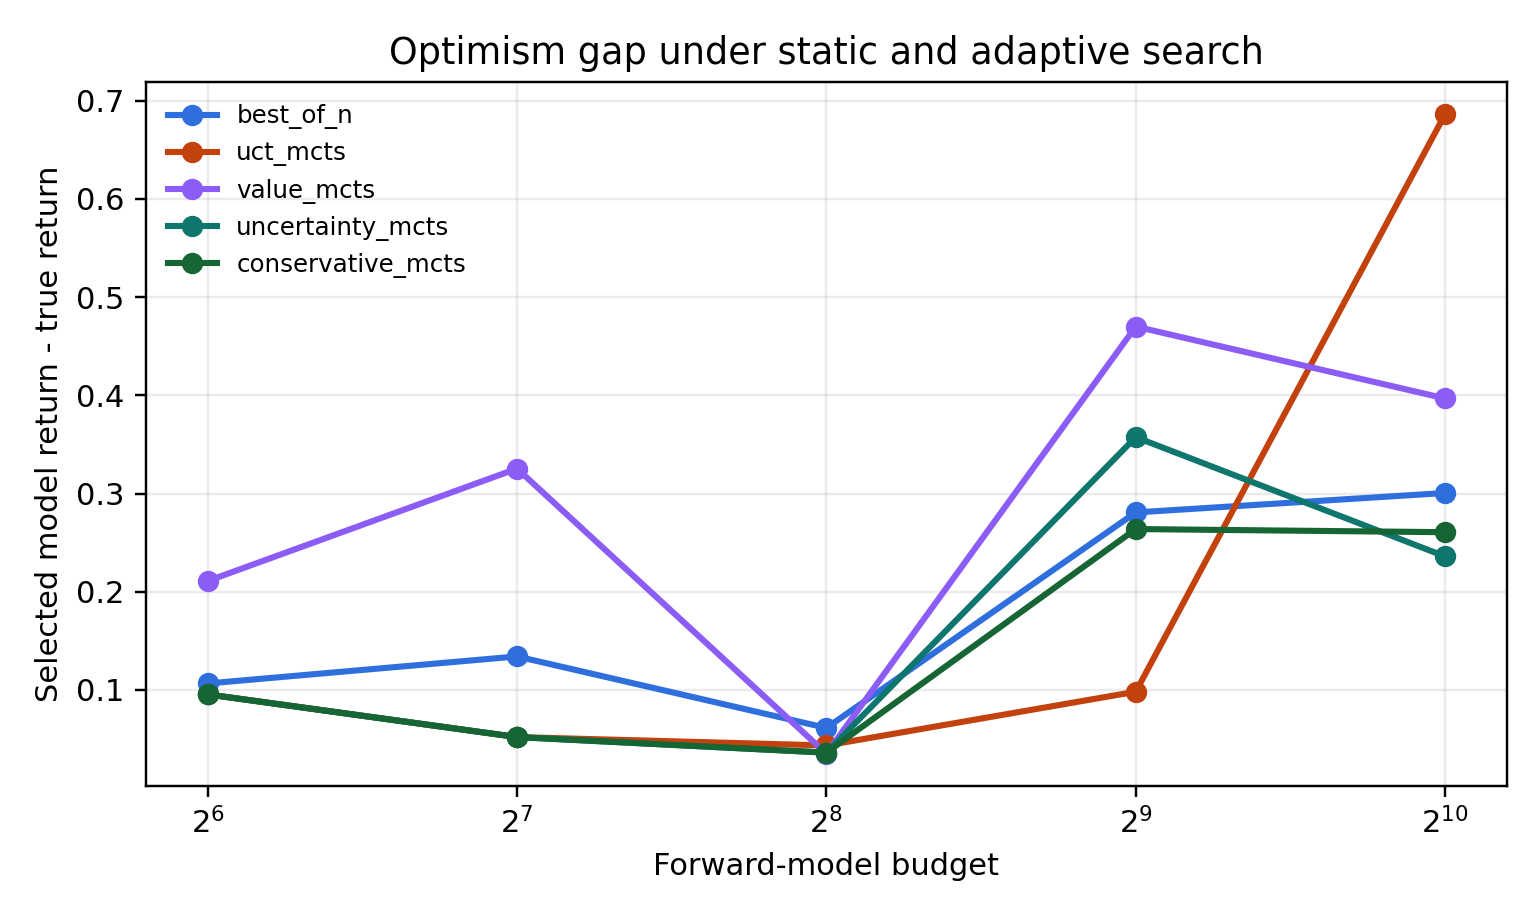
\includegraphics[width=0.92\linewidth]{compute_scaling.png}
\caption{Selected-return optimism gap across forward-model budgets.}
\end{figure}

\begin{figure}[h]
\centering
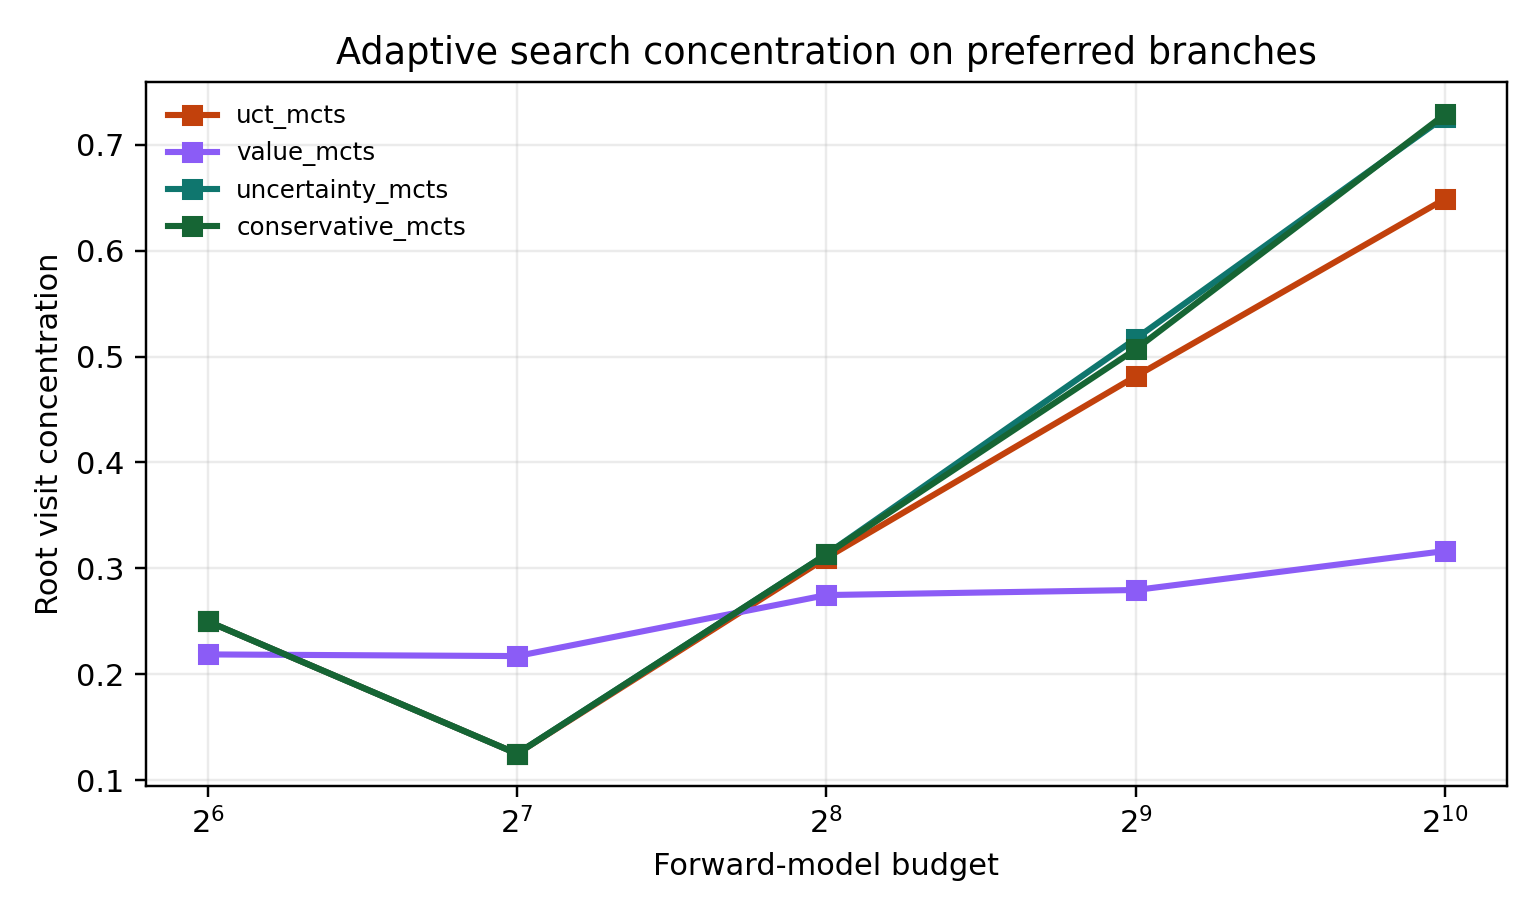
\includegraphics[width=0.92\linewidth]{bias_amplification.png}
\caption{Root visit concentration increases as adaptive tree search allocates budget to preferred branches.}
\end{figure}

\begin{figure}[h]
\centering
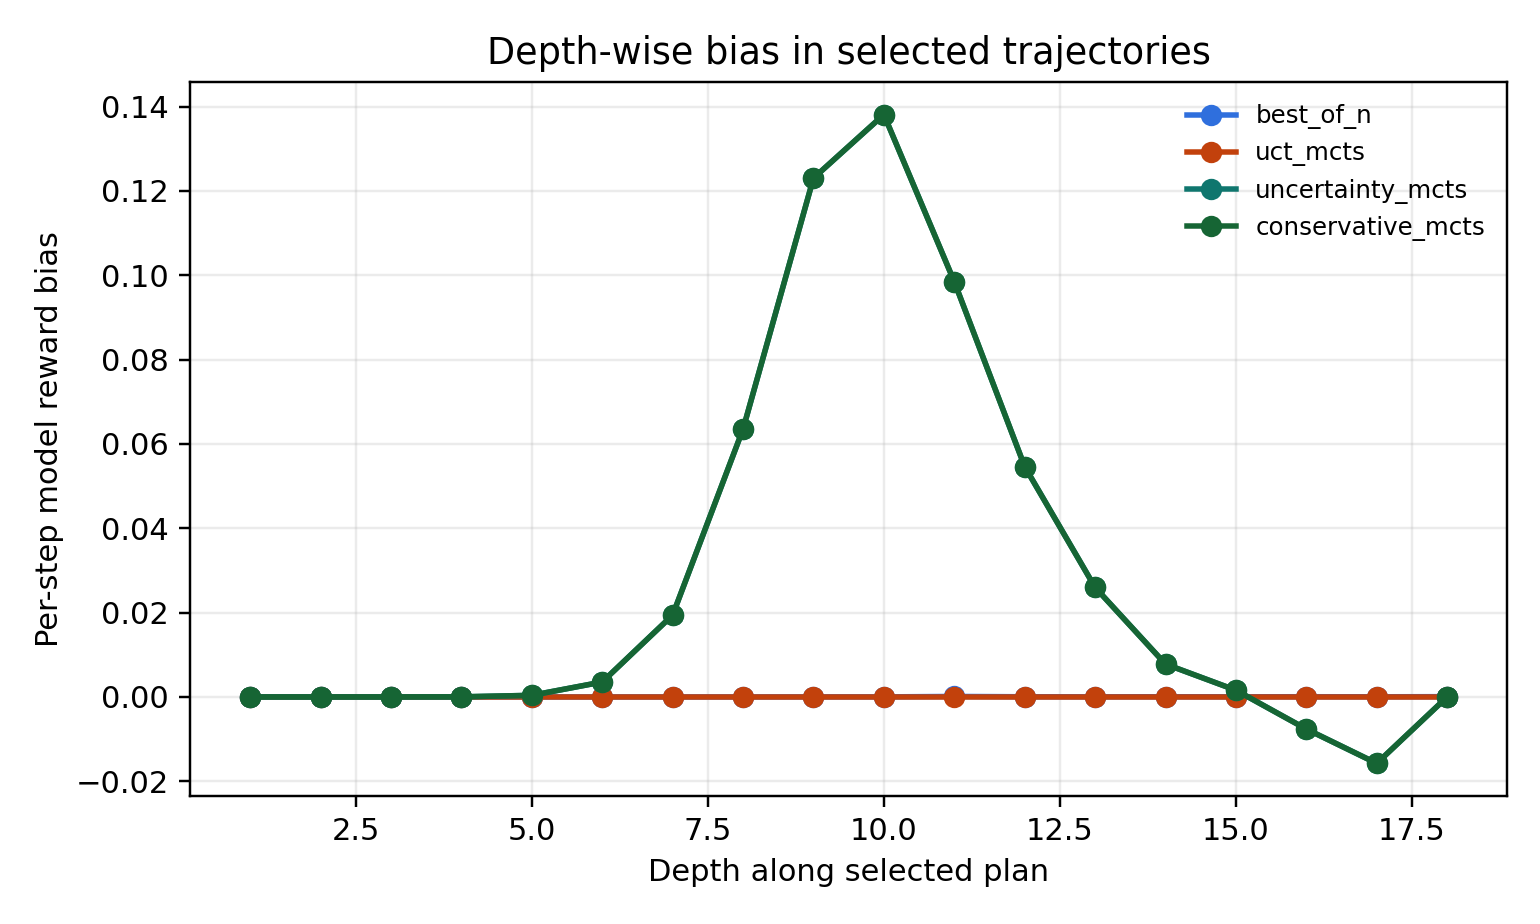
\includegraphics[width=0.92\linewidth]{depth_bias_profile.png}
\caption{Depth-wise learned reward bias along selected plans in the largest-budget run.}
\end{figure}

\section{Interpretation}

The result supports the narrow mechanism claim: in this controlled model, adaptive tree search can select trajectories whose learned return is more optimistic than the trajectories selected by static best-of-N under equal model-step budgets. The uncertainty-calibrated variants reduce the selected-return gap in the largest-budget run.

The result should not be overclaimed. The learned model is hand-designed rather than trained. The uncertainty signal is intentionally aligned with the injected bias pocket. The experiment is a microscope, not a benchmark. Its value is that the failure mode is observable, testable, and easy to extend.

\section{Limitations and Next Steps}

The next version should train an ensemble dynamics model on biased data, add continuous-action expansion, and evaluate on at least one standard continuous-control benchmark. The repair should be stress-tested under miscalibrated uncertainty and value-function optimism. The most important open question is whether search concentration predicts real downstream regret when the learned model is trained rather than hand-specified.

\bibliographystyle{plain}
\bibliography{references}

\end{document}
